%!TEX root = main.tex
% UTF-8 encoding
\section{Discussion}
\label{sec:dis}
The discussion is primarily conducted for the drug dataset considering that euphemisms for drug are vast and evolve more rapidly. 


\subsection{Case Studies on Euphemism Detection}

\begin{table*}
	\centering
	\caption{Euphemism detection results by our approach (better viewed in color). 
		Purple bold words are correctly detected euphemisms and on the ground truth list (\ie, the DEA list). 
		The purple underlined words indicate that they are incorrect by themselves, but are contained in true euphemism phrases, such as ``dog food", ``Chinese Tabacco" (euphemisms for ``heroin" and ``opium" respectively). 
		Those words which do not appear in the ground truth list are marked black. 
		}
	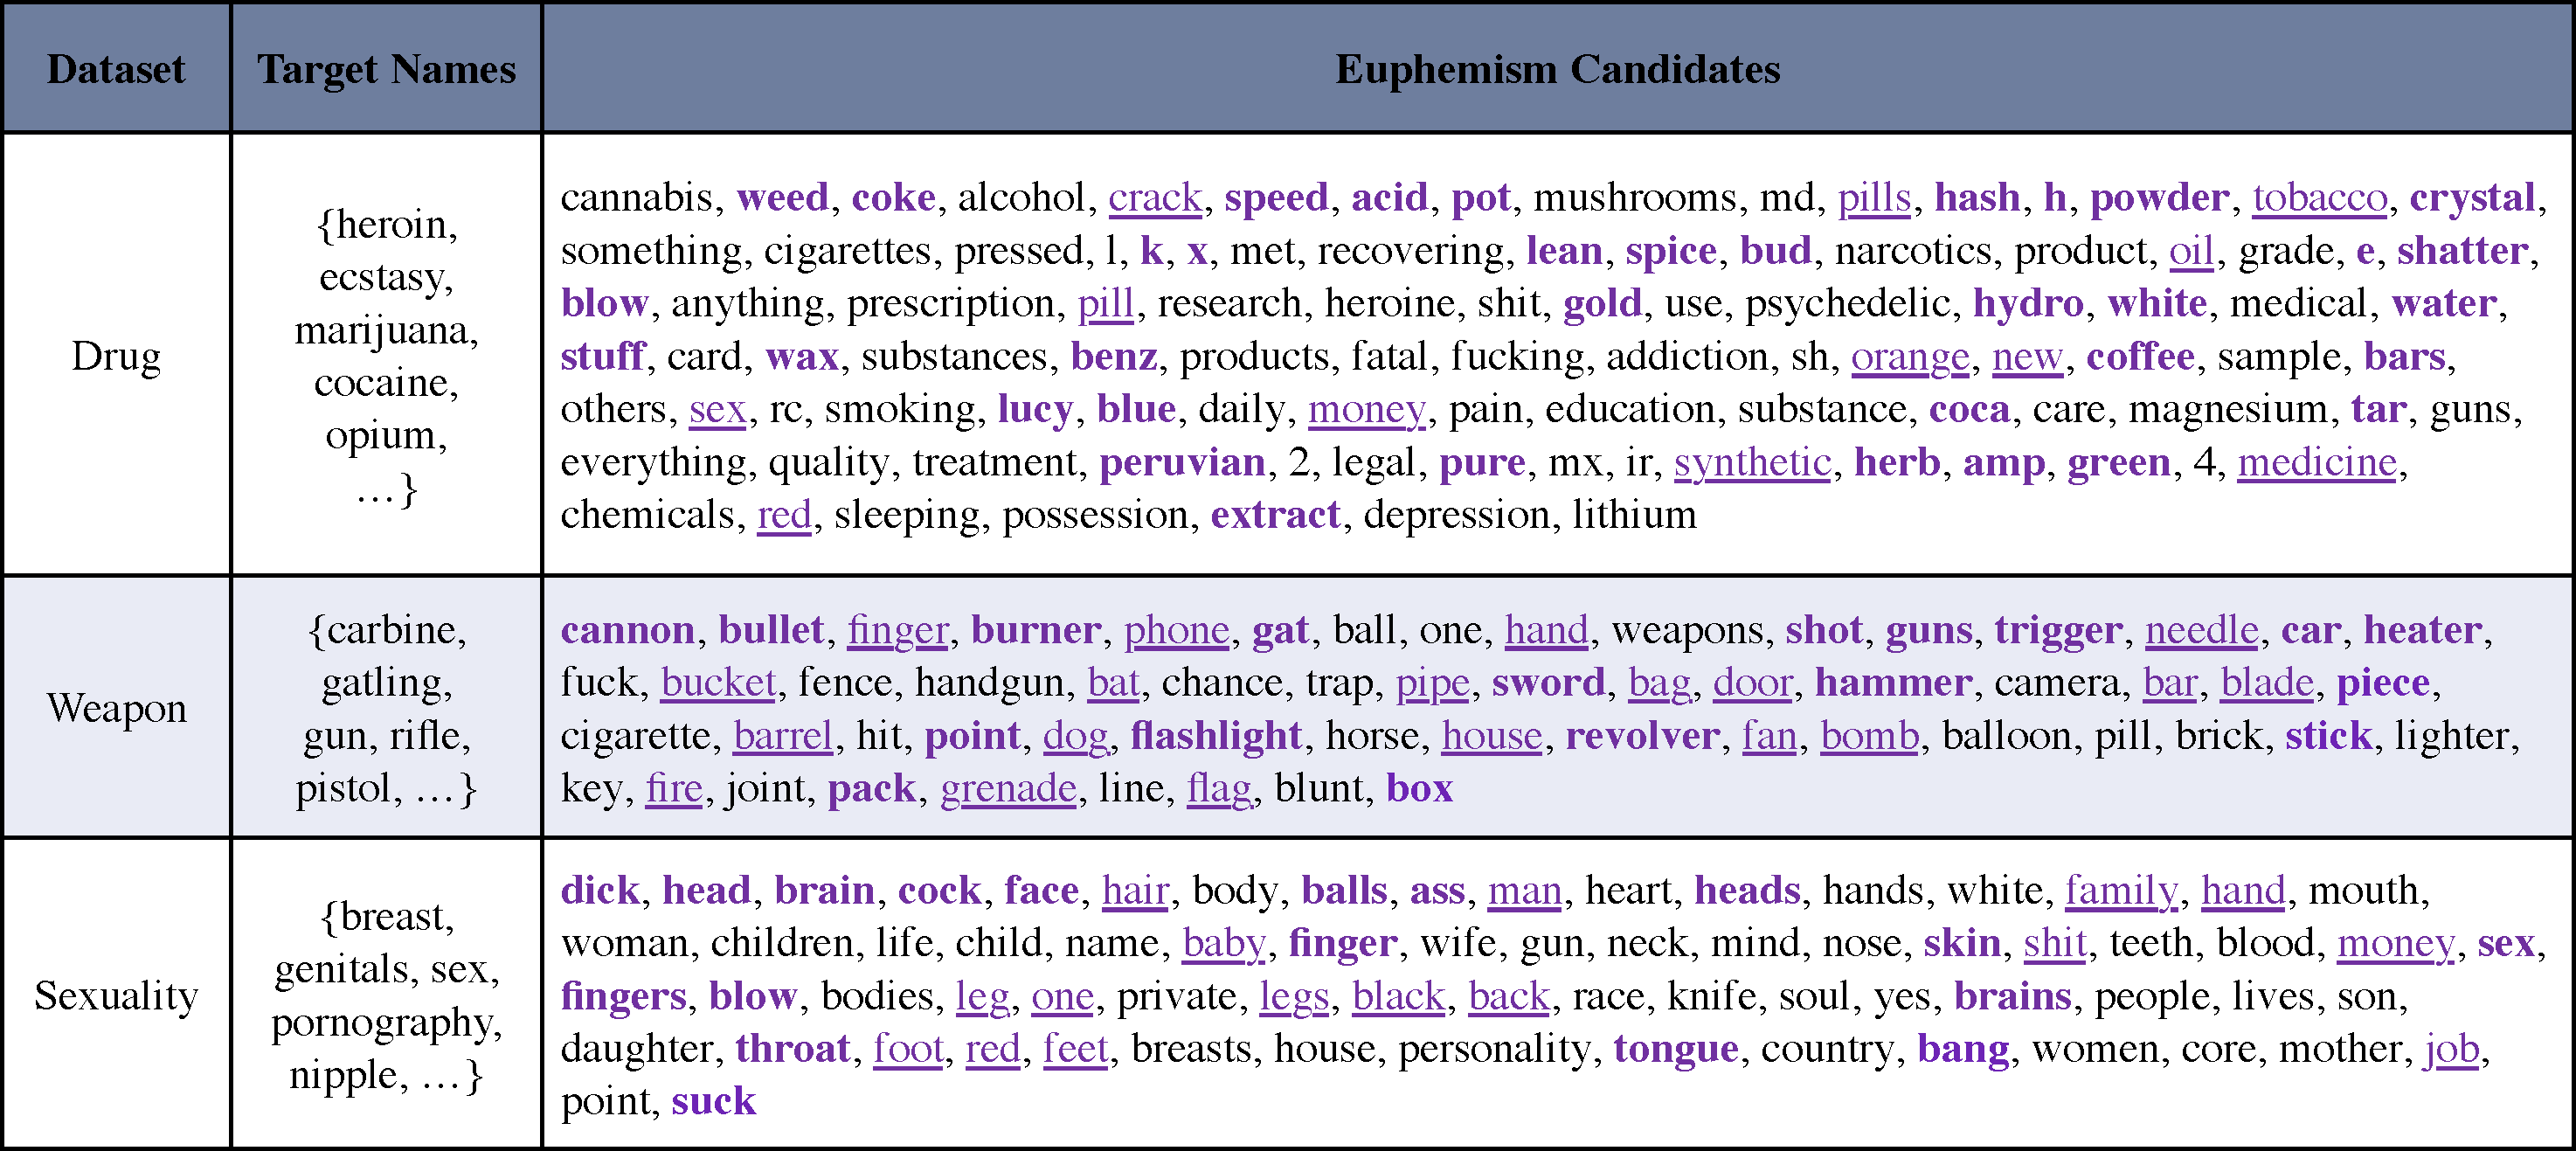
\includegraphics[width=1\linewidth]{figures/CaseStudies-Detection}
	\label{fig:casestudies-detection}
\end{table*}

\begin{table*}
	\centering
	\caption{Case studies of the false positive detection results on the drug dataset. They are real examples from Reddit.}
	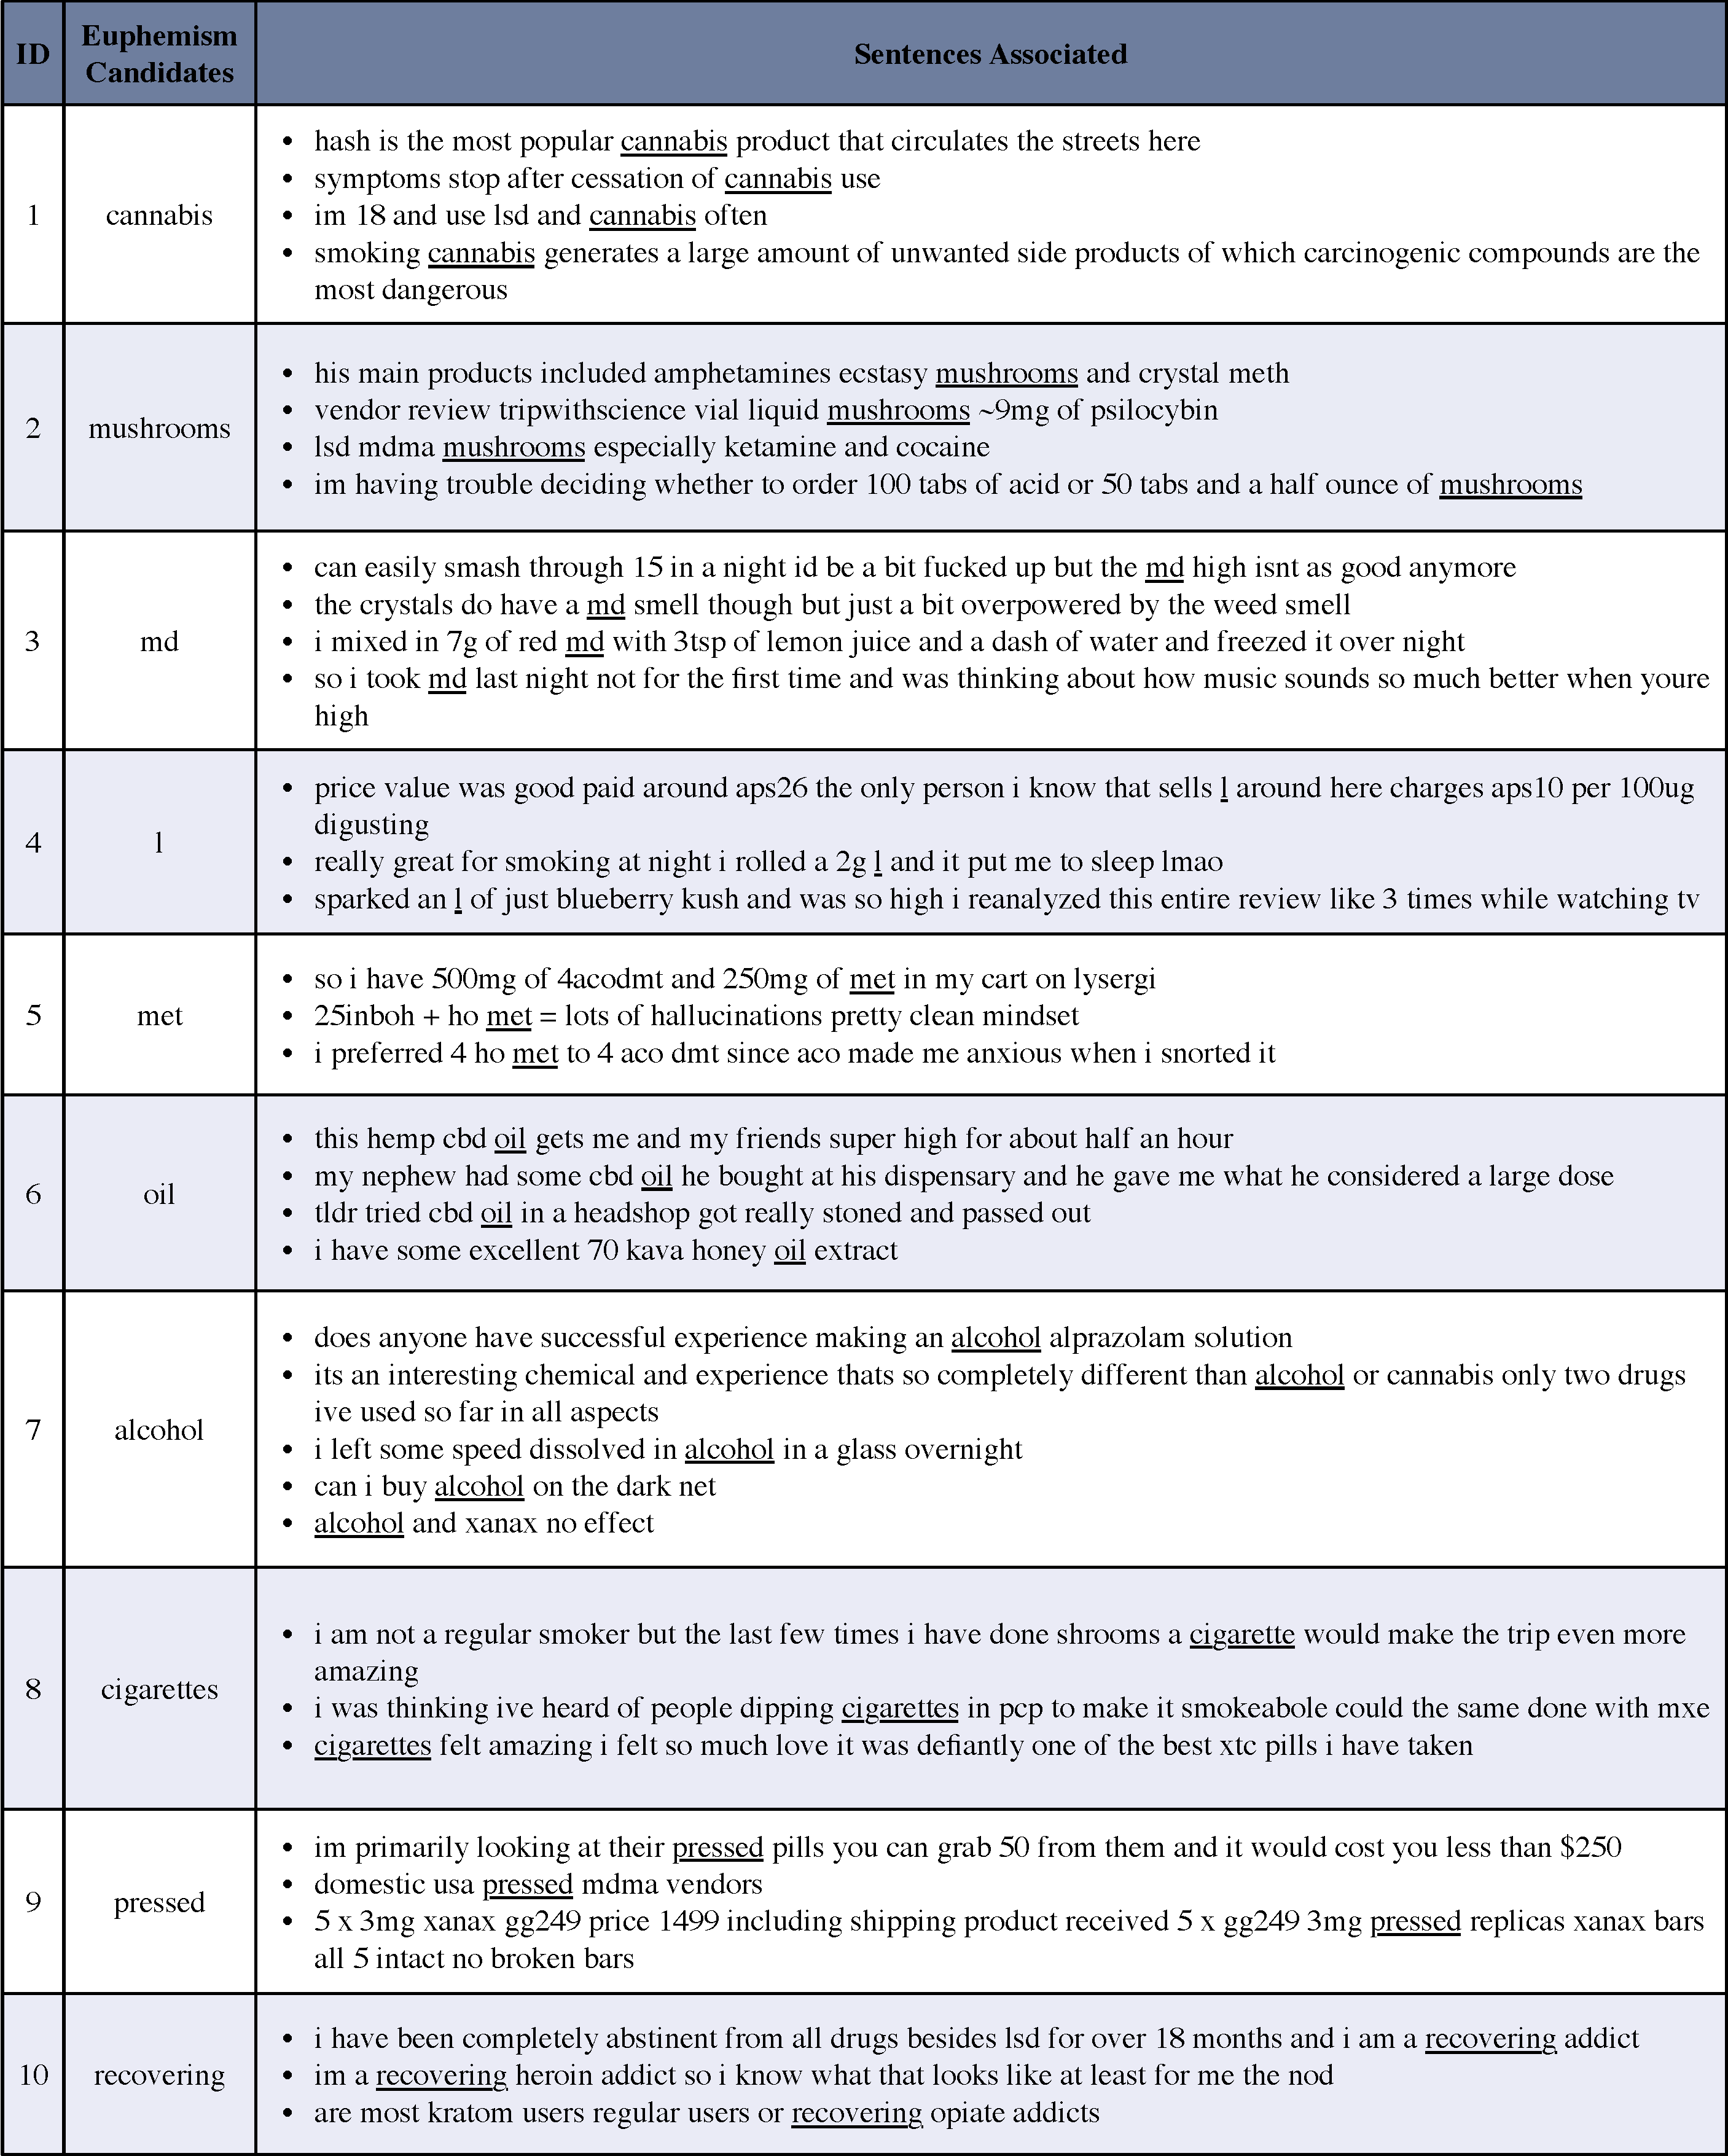
\includegraphics[width=1\linewidth]{figures/CaseStudies-Detection2}
	\label{fig:casestudies-detection2}
\end{table*}

We present the euphemism detection results by our approach in Table \ref{fig:casestudies-detection} and analyze the false positive detection results on the drug dataset in Table \ref{fig:casestudies-detection2}. 
We categorize our false detection results into four types: 
\begin{itemize}
	\item They are correct euphemisms but missed on the ground truth list (cases 1-5 in Table \ref{fig:casestudies-detection2}). 
	\item They are not euphemisms by themselves, but they are contained in euphemism phrases. For example, as shown in case 6 in Table \ref{fig:casestudies-detection2}, ``crack'' is not a drug euphemism while ``green crack'' is one. 
	\item Though they are not euphemisms, they are strongly related to drug or the usage of drug (cases 7-10 in Table \ref{fig:casestudies-detection2}). Cases 7 and 8 uncovers some ways that people take drugs (together with alcohol or cigarettes).
	\item Incorrect detection. 
\end{itemize}

The case studies reveal that we can even find some correct euphemisms that are not on the ground truth list, which suggests the rapid-evolving nature of euphemisms and the necessity of the automatic euphemism detection task. 




\subsection{Ablation Studies for Euphemism Identification}
We adopt a coarse-to-fine-grained classification scheme for euphemism identification. 
We discuss the performance of multiple classifiers on both coarse and fine-grained classification. 

\subsubsection{Coarse Classifiers}
\label{sec:ablation_coarse}
\begin{figure}[ht!]
	\centering
	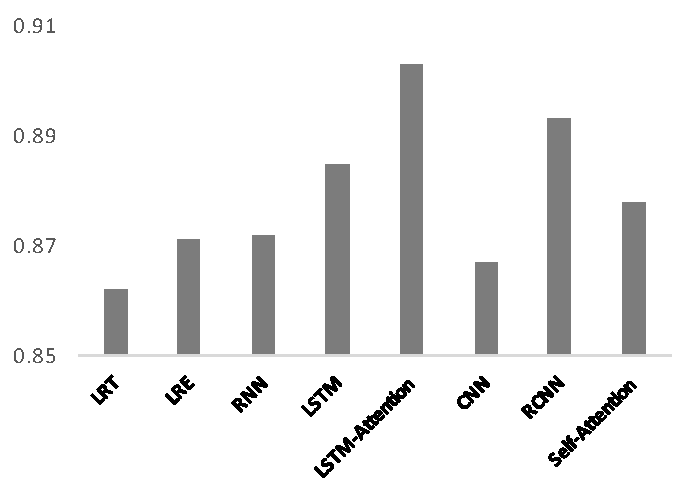
\includegraphics[width=0.7\linewidth]{figures/11}
	\caption{Testing accuracy for the coarse classifier.}
	\label{fig:11}
\end{figure}

In the euphemism identification framework, we use a binary classifier to filter out the sentences where euphemisms are used in non-euphemistic senses. 
We experiment with the following binary classifiers: 
\begin{itemize}
	\item Logistic Regression on raw text (LRT): we represent each word by one-hot encoding and the sentence by the average of the composing words' encoding. 
	\item Logistic Regression on text embeddings (LTE): we learn the word embeddings using word2vec \cite{mikolov2013distributed,mikolov2013efficient}. The sentence embedding is the average of the composing words' embeddings. 
	\item Recurrent Neural Network (RNN) \cite{rumelhart1985learning}
	\item Long Short-Term Memory (LSTM) \cite{hochreiter1997long}
	\item LSTM-Attention: we add an attention mechanism \cite{bahdanau2015neural} on LSTM. 
	\item Convolutional Neural Networks (CNN) \cite{kim2014convolutional}
	\item Recurrent Convolutional Neural Networks (RCNN) \cite{lai2015recurrent}
	\item Self-Attention \cite{lin2017structured}
\end{itemize}

We split the datasets into 70-10-20 for training, validating and testing. 
The model parameters are tuned on the validation data. 
Empirically, we find the LSTM with attention performs the best across three datasets. 
Yet as shown in Figure \ref{fig:11}, other classifiers have satisfactory performance as well and reaching a testing accuracy from 0.86 to 0.90. 



\subsubsection{Fine-Grained Classifiers}
\label{sec:ablation_fine-grained}
In the euphemism identification framework, we use a multi-class classifier to identify to which target keyword each euphemism refers. 
Again, we experimented with the same set of classifiers in Section \ref{sec:ablation_coarse}. 
Interestingly, we find that all classifiers have highly similar results. 
We think one possible reason is that each class has relatively small number of training instances (ranging from a few hundreds to 100k), which limits the discriminative power of advanced algorithms. 
For the drug dataset (33 target keywords), the training accuracy is about 55\% and the testing accuracy is about 24\%. 
This shows the feasibility of the task since the random guess accuracy would be 3.3\%. 
Given the similar performance across different classifiers, we recommend using Logistic Regression on raw text for better computational efficiency. 




\subsection{Parameter Analysis}
\label{sec:dis_parameter_analysis}
\begin{figure}[ht!]
	\centering
	%\vspace{-0.5cm}
	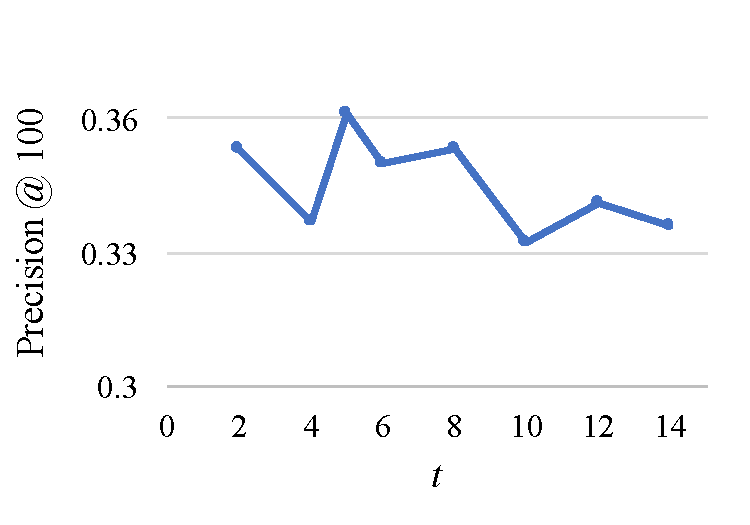
\includegraphics[width=0.6\linewidth]{figures/12}
	\caption{Sensitivity of $t$.}
	\label{fig:12}
\end{figure}

In the euphemisms detection step (Section \ref{sec:model_det}), we set an masked language model threshold $t$ to filter out the generic masked sentences. 
Considering the ranked list of replacements for the mask token, if any target keyword appears in the top $t$ replacement candidates for the masked sentence, we consider  the masked sentence to be a valid instance of a context. Otherwise, it is considered to be a generic one and will be filtered out. 
Figure \ref{fig:12} shows how the results change with the threshold $t$ and we observe a slight decrease when the threshold $t$ is larger than 5. 







% Detection Challenges
% Identification Challenges




%\subsection{Limitation and Future Work}
%%We run our experiments on two other datasets with relatively negative results. 
%Euphemistic phrase detection. 




%\subsection{The Effect of Fine-tuning the BERT Model}
%\begin{figure}[ht!]
%	\centering
%	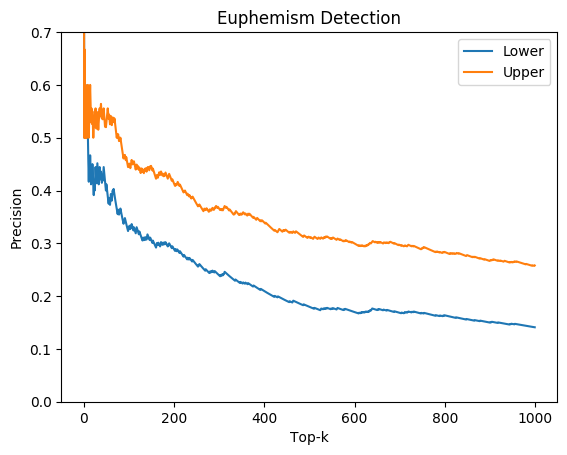
\includegraphics[width=0.48\linewidth]{figures/Precision_reddit}
%	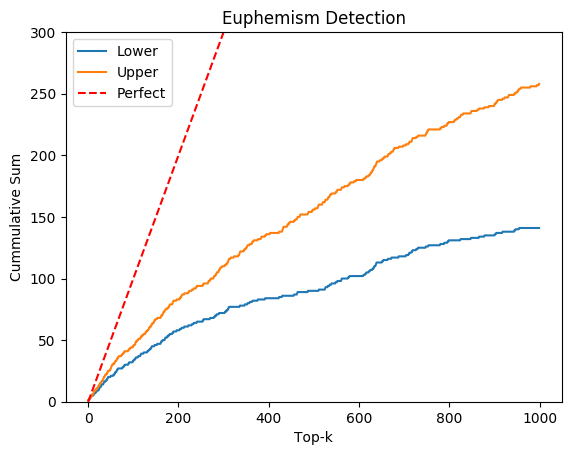
\includegraphics[width=0.48\linewidth]{figures/CSum_reddit}
%	\caption{Left shows the top-k precision \textit{vs.} k on the drug dataset. Right shows the cumulative correct numbers \textit{vs.} k on the drug dataset. }
%	\label{fig:precisionreddit}
%\end{figure}
%We have shown the numeric results of euphemism detection in Table \ref{table:res_dec}. Besides, we show the plots on top-k precision and cummulative correct detections against k in Figure \ref{fig:precisionreddit}. 



%\subsection{Computational Efficiency}
%We did not measure the baselines so far. 
%We implemented all models in Python 3.7 and conducted all the experiments on a computer with twenty 2.9 GHz Intel Core i7 CPUs and one GeForce GTX 1080 Ti GPU. 
%The BERT fine-tuning on the text corpus step took 5.4 hours (3 epochs).
%The euphemism detection took 1.5 hours. 
%The euphemism identification took 1.5 hours. 

